Le projet est sur de bonnes voies, mais il reste encore un long travail pour faire de ce prototype un modèle fonctionnel. Nous avons réfléchi a différents axes d'amélioration, que nous implémenterons si nous avons le temps.

Voici une liste des améliorations possibles, sans ordre de priorité particulier :

\vspace{0.5cm}
\begin{enumerate}
	\item \textbf{Modifier les textures du programme afin d'adopter un rendu "`Lego"'} : Notre choix s'est volontairement porté sur un rendu à la \textit{Minecraft}, le jeu étant lui-même inspiré de la marque Lego. Notre but sera donc, ou bien de trouver des textures de remplacement sur le Net, ou bien de créer nos propres textures.
	\item \textbf{Améliorer la structure du code :} Nous ne disposons pour le moment que d'un prototype issu de recherches, de tâtonnements et d'assemblages. A terme, nous souhaiterions donner une meilleure lisibilité au code du projet, voire pourquoi pas de créer notre propre interface paramétrable, comme il en existe dans certains projets de three.JS.
	\item \textbf{Rendre le personnage visible} : L'intérêt du projet est également de représenter un personnage évoluant dans l'univers généré. Son apparence reste encore à décider.
	\item \textbf{Donner de la solidité au terrain }: Actuellement, l'univers modélisé n'a pas de consistance : le joueur peut travers le terrain comme il le souhaite. L'idée serait de rendre ce terrain concret et infranchissable.
	\item \textbf{Rajouter une surcouche physique }: Pour l'heure, three.JS permet au joueur de voler et de se déplacer dans l'univers comme il l'entend. Un point intéressant à rajouter serait de rajouter de la gravité ainsi qu'un système de sauts, afin de rendre l'expérience plus réaliste et proche des jeux existants.
	\item Changer les textures en fonction de l'altitude: L'API que nous avons utilisée n'est fournie qu'avec un seul type de textre (de l'herbe.) Il pourrait être intéressant de faire varier le type de terrain exploré par le joueur.
	\item \textbf{Se déplacer avec ZQSD} : Le déplacement avec la souris et les flèches directionnelles est peu pratique. Changer les touches de déplacement afin d'instaurer une maniabilité classique avec ZQSD serait un plus.
	\item \textbf{Implémenter génération de terrain avec le bruit de Simplex }: Le bruit de Simplex étant la version évoluée et plus moderne du bruit de Perlin, il serait intéressant de se pencher dessus afin de saisir les différences entre ces deux algorithmes, et d'observer le résultat sur notre carte en 3D. 
	\item \textbf{Ajouter divers éléments de décors }(arbres, cours d'eau, etc.) : L'univers généré est pour le moment vide et fade. Y ajouter des éléments ponctuels lui donnerait un peu plus de vie et de réalisme.
\end{enumerate}
\vspace{0.5cm}

\begin{center}
	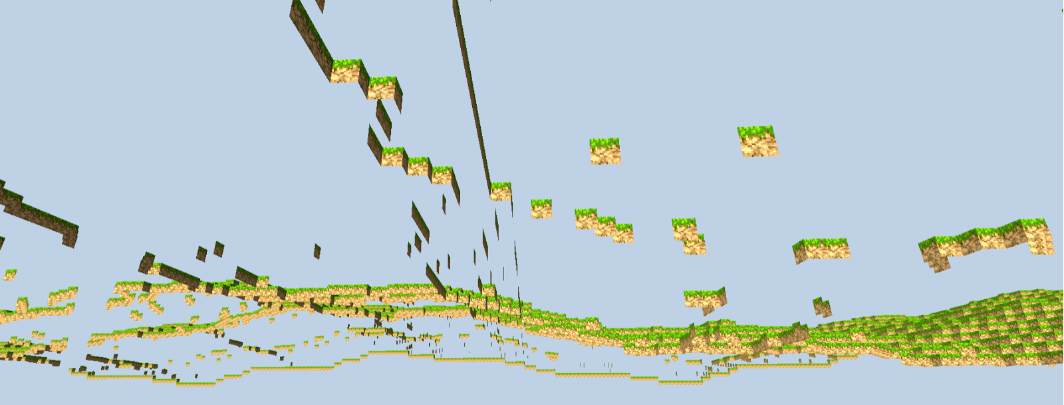
\includegraphics[height=6cm]{images/screen_fail.png}\\
	\textit{Exemple de ce qui se passe quand on franchit le sol.}
\end{center}







